\graphicspath{{Podkopaev/images/}}

\lstdefinelanguage{llang}{
	keywords={skip, do, while, read, write, if, then, else},
	sensitive=true,
	%%basicstyle=\small,
	commentstyle=\scriptsize\rmfamily,
	keywordstyle=\ttfamily\underbar,
	identifierstyle=\ttfamily,
	basewidth={0.5em,0.5em},
	columns=fixed,
	fontadjust=true,
	literate={->}{{$\to$}}1
}

\lstset{
	language=llang
}

\title{Форматирование текста программ\\ 
на основе комбинаторов,\\
сопоставления с образцом\\
и синтаксических шаблонов}
%
\titlerunning{Форматирование текста программ}
\author{Подкопаев Антон Викторович}
%
\authorrunning{А.В.Подкопаев} % abbreviated author list (for running head)
%
%%%% list of authors for the TOC (use if author list has to be modified)
\tocauthor{А.В.Подкопаев}
%
\institute{Санк-Петербургский государственный университет\\
\email{podkoav239@gmail.com}}

\maketitle              % typeset the title of the contribution

\begin{abstract}
\end{abstract}
%

\section*{Введение}

Ручное управление памятью в языках, подобных C++, является источником большого количества трудно отслеживаемых ошибок, наличия которых можно было бы
избежать, сделав процесс управления памятью автоматическим. \textit{Сборка мусора} является одним из способов автоматического управления памятью, при
котором освобождение памяти выводится из-под контроля ПО на прикладном уровне. При автоматическом управлении программист не может явно влиять на распределение
объектов в памяти, у него есть лишь
косвенные способы сделать это с помощью использования тех или иных языковых конструкций. В идеальном случае, для рационального использования
памяти необходимо освобождать память, занимаемую объектами, которые более не будут использованы программой. Поскольку точно определить, что
объект не будет использован в дальнейшем, невозможно, на практике используют критерий доступности. \textit{Доступность} --- это консервативное
приближение используемости. \textit{Мусором}, в таком случае, называют объект, все пути доступа к которому уже разрушены, а память из-под него
ещё не освобождена. В некоторое, заранее определенное время, например, в простейшем случае, когда перестаёт хватать свободной памяти, выполнение
программы временно приостанавливается и запускается процесс \textit{сборки мусора}, который освобождает всю или ту, что возможно, память,
занятую мусором, после чего управление возвращается обратно программе. \textit{Сборщиком мусора} называется компонент, производящий \textit{сборку мусора}.

Процесс \textit{сборки мусора}, в простейшем случае, делят на три этапа:
\begin{enumerate}
\item \textit{Построение корневого множества}. На этом этапе строится множество объектов, которые считаются изначально доступными.
Такие объекты называются \textit{корнями} (англ. roots). Данное построение
аксиоматично, т.е. основывается на некотором наборе правил, согласно которым те или иные элементы считаются доступными. Данный этап является неотъемлемой
частью любого сборщика мусора.
\item \textit{Маркировка}. Начиная с множества, построенного на предыдущем этапе, происходит сканирование памяти, и все объекты, до которых возможно
добраться из построенного корневого множества, считаются доступными; оставшиеся объекты считаются мусором.
\item \textit{Освобождение}. Происходит сканирование кучи, в течение которого память из-под всех элементов, помеченных как мусор или не отмеченных как
доступные, освобождается.
\end{enumerate}

Есть несколько требований, которые должны быть выполнены для реализации сборки мусора:
\begin{enumerate}
\item Возможность построения корневого множества. Иными словами, необходимо иметь возможность идентифицировать все указатели в программном стеке, регистрах
и статической области памяти.
\item Должна присутствовать возможность определить все указатели из любого объекта на другие элементы кучи.
\end{enumerate}
В таких языках, как LISP или JAVA все условия соблюдаются, и в них успешно используется технология сборки мусора, в то время как, например,
в языке C не все условия выполняются. В языках, где не соблюдаются хотя бы одно из вышеперечисленных условий, возможна исключительна
\textit{консервативная сборка мусора}.
\textit{Консервативной} называется такая сборка мусора, при которой любой элемент данных, значение которого может быть истолковано, как указатель на
некоторый элемент кучи, считается  таковым. Консервативный подход к сборке мусора не позволяет собрать весь мусор, что может стать проблемой при обработке
большого количества данных. Неконсервативная сборка мусора лишена подобного недостатка и способна освободить всю память программы, более не
являющуюся доступной. \textit{Неконсервативным} или  \textit{точным сборком мусора} называется сборщик мусора, имеющий возможность точно распознать
все указатели в памяти. Иными словами, точный сборщик мусора --- это сборщик мусора, не использующий консервативный подход.

В C++ не соблюдаются требования, необходимые для сборки сборки мусора, реализовать точный сборщик мусора без ограничений
на использование некоторых примитивов языка не представляется возможным.
Более того, в C++ имеется ряд технических сложностей, затрудняющих реализацию точного сборщика мусора.
Тем не менее, в случае соблюдения программистом некоторых соглашений на програмный код,
точная сборка мусора становится возможной и в C++.

Целями работы является реализация основных примитивов библиотеки неконсервативной сборки мусора для C++,
обеспечение возможности совмещения ручного и автоматического управления памятью.
\section{Обзор существующих библиотек}

В рамках исследования был проведен анализ основных существующих функциональных принтер-библиотек. Все выбранные библиотеки оказались комбинаторными, что естественно для функциональных языков.

% Так как работа проводилась в контексте функциональных языков, для анализа были выбраны комбинаторные библиотеки.
% Комбинаторы естественным образом возникают при наличии в языке функций высших порядков.

\subsection{Модельный язык L}
% \addcontentsline{toc}{section}{Модельный язык L}

В дальнейшем центральным примером, для которого мы будем разрабатывать принтеры, будет модельный язык L. Именно для этого языка будет реализован шаблонный принтер.

Язык L состоит из небольшого числа операторов:
\begin{enumerate}
	\item присваивание;
	\item цикл с предусловием;
	\item ветвление;
	\item последовательное выполнение;
	\item чтение с занесением в переменную;
	\item печать целочисленного выражения.
\end{enumerate}

Также в языке есть выражения. Выражения бывают трех типов:
\begin{enumerate}
	\item константа;
	\item переменная;
	\item бинарная операция.
\end{enumerate}

На рисунке~\ref{fig:lEx} приведен пример программы на языке L. В данном случае, это программа, которая считывает с консоли два числа, а потом возводит второе число в степень, равную первому.

\begin{figure}[h!]
	\centering
	% \inputminted{pascal}{codes/lEx.l}
	\lstinputlisting[language=llang]{codes/lEx.l}
	\caption{Быстрое возведение в степень на языке L}
	\label{fig:lEx}
\end{figure}

\subsection{Библиотека Хьюза}

Библиотека Джона Хьюза\cite{hughes} считается первой комбинаторной принтер-библиотекой. Она основана на алгоритме, предложенном Дереком Оппеном \cite{oppen}, и по сути является его реализацией в функциональном стиле на языке Haskell\footnote{http://haskell.org}. Также библиотека Хьюза, расширенная Саймоном Пейтоном Джонсом \cite{peytonJones}, является стандартной принтер-библиотекой для языка Haskell.

% рассказать об оптимальном

В данной библиотеке ключевым типом является “\lstinline[language=Haskell]{Doc}”. Он представляет документ, который потом может быть переведен в строковое представление.
Основные комбинаторы для составления документа:
% \inputminted{haskell}{Podkopaev/codes/hughesBasicOperators.hs}
\lstinputlisting[language=Haskell]{Podkopaev/codes/hughesBasicOperators.hs}

Так, с помощью функции “\lstinline[language=Haskell]{text}” по строке получается документ, оператор “\textbf{<>}” соединяет два документа горизонтально (см. рисунок~\ref{fig:hughesHorComp}), а оператор “\textbf{\$\$}” соединяет документы вертикально (см. рисунок~\ref{fig:hughesVertComp}).

\begin{figure}[ht]
	\begin{subfigure}[b]{0.45\linewidth}
		\centering
		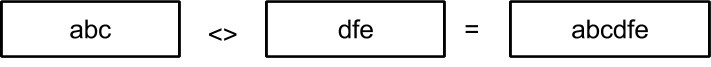
\includegraphics[width=\textwidth]{hughesHorComp}
		\caption{Комбинатор “\textbf{<>}”}
		\label{fig:hughesHorComp}
	\end{subfigure}
	\hspace{0.5cm}
	\begin{subfigure}[b]{0.45\linewidth}
		\centering
		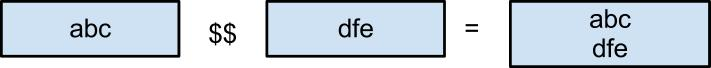
\includegraphics[width=\textwidth]{hughesVertComp}
		\caption{Комбинатор “\textbf{\$\$}”}
		\label{fig:hughesVertComp}
	\end{subfigure}

	\caption{Пример работы комбинаторов}
\end{figure}

Функция “\lstinline[language=Haskell]{nest}” добавляет к каждой строке документа заданное число ведущих пробелов. Функция “\lstinline[language=Haskell]{sep}” является ключевым комбинатором, который в этой библиотеке позволяет задавать плавающую раскладку документа. Она принимает как параметр список документов, а на выходе получается документ, который представляет из себя либо вертикальную склейку элементов списка, либо горизонтальную склейку (в этом случае если к документу из списка применялась функция “\lstinline[language=Haskell]{nest}”, то к этому документу не добавляются ведущие пробелы, то есть применение “\lstinline[language=Haskell]{nest}” попросту игнорируется), причем между документами вставляется пробельный символ. Вариант раскладки выбирается функцией “\lstinline[language=Haskell]{pretty}”:

% \inputminted{haskell}{Podkopaev/codes/hughesPretty.hs}
\lstinputlisting[language=Haskell]{Podkopaev/codes/hughesPretty.hs}

Кроме самого документа, функция “\lstinline[language=Haskell]{pretty}” также принимает два числа: максимальную длину и максимальную наполненность строки. Здесь наполненность строки значит длину текста без ведущих пробельных символов. В ходе работы этой функции и происходит выбор раскладки документа, полученного с помощью комбинатора “\lstinline[language=Haskell]{sep}”. Если горизонтальная раскладка удовлетворяет ограничениям на ширину строки, то она и выбирается. Иначе выбирается вертикальная раскладка.


% Возможно, стоит сделать после обзора всех библиотек

Рассмотрим пример описания принтера с помощью библиотеки Хьюза. Для этого используем учебный язык L. Часть принтера для языка L, отвечающая за представление операторов, показана на рисунке~\ref{fig:lHughesPrinter}.
В примере используется не описанный выше комбинатор “\lstinline[language=Haskell]{<+>}”, который определяется следующим образом:

\lstinputlisting[language=Haskell]{Podkopaev/codes/hughesAddComb.hs}

\begin{figure}[h!]
	% \inputminted{haskell}{Podkopaev/codes/lHughesPrinter.hs}
	\lstinputlisting[language=Haskell]{Podkopaev/codes/lHughesPrinter.hs}
	\caption{Принтер, написанный с помощью библиотеки Хьюза}
	\label{fig:lHughesPrinter}
\end{figure}

В данном случае принтер получился несложным, но абсолютно не наглядным. Поскольку в библиотеке нет механизмов, позволяющих явно варьировать раскладку документа в зависимости от раскладки его поддокументов, невозможно выразить пример с рисунка~\ref{fig:lGoodWriteEx}.
То есть, в случае многострочного выражения в операторе “\lstinline[language=llang]{write}”, напечатать закрывающую скобку на уровне самого оператора.

\begin{figure}[h!]
	% \inputminted{pascal}{Podkopaev/codes/lGoodWriteEx.l}
	\lstinputlisting[language=llang]{Podkopaev/codes/lGoodWriteEx.l}
	\caption{Желательный пример печати конструкции “\lstinline[language=llang]{write}”}
	\label{fig:lGoodWriteEx}
\end{figure}

С помощью реализации принтера с рисунка~\ref{fig:lHughesPrinter}, в данном случае для оператора “\lstinline[language=llang]{write}” получится немного не то (см. рисунок~\ref{fig:lCurWriteEx}).
\begin{figure}[h!]
	% \inputminted{pascal}{Podkopaev/codes/lCurWriteEx.l}
	\lstinputlisting[language=llang]{Podkopaev/codes/lCurWriteEx.l}
	\caption{Результат для изначального принтера конструкции “\lstinline[language=llang]{write}”}
	\label{fig:lCurWriteEx}
\end{figure}

Если попробовать поменять функцию “\lstinline[language=Haskell]{docFromOperation}” для конструкции “\lstinline[language=llang]{write}” (см. рис. \ref{fig:lHughesWriteChange}),
то для многострочного выражения все получится правильно, но в случае однострочного --- появится лишний пробел перед закрывающей скобкой (см. рис. \ref{fig:lBadWriteEx})).

\begin{figure}[h!]
	% \inputminted{haskell}{Podkopaev/codes/lHughesWriteChange.hs}
	\lstinputlisting[language=Haskell]{Podkopaev/codes/lHughesWriteChange.hs}
	\caption{Измененный принтер конструкции “\lstinline[language=llang]{write}”}
	\label{fig:lHughesWriteChange}
\end{figure}

\begin{figure}[h!]
	% \inputminted{pascal}{Podkopaev/codes/lBadWriteEx.l}
	\lstinputlisting[language=llang]{Podkopaev/codes/lBadWriteEx.l}
	\caption{Результат для измененого принтера конструкции “\lstinline[language=llang]{write}”}
	\label{fig:lBadWriteEx}
\end{figure}
\newpage

\subsection{Принтер-комбинаторная библиотека Вадлера}

В \cite{wadler} Филипп Вадлер описал свою комбинаторную бибилиотеку для форматированного вывода на языке Haskell. Она является модификацией библиотеки Хьюза, описанной в предыдущем разделе. Код библиотеки сократился с $\approx$ 110 строк до $\approx$ 80 строк, и, по исследованию Вадлера, на 30\% увеличилась скорость вычисления раскладки документа.

Рассмотрим основые комбинаторы этой библиотеки:
% \inputminted{haskell}{codes/wadlerBasicOperations.hs}
\lstinputlisting[language=Haskell]{codes/wadlerBasicOperations.hs}

Вадлер решил отказаться от двух разных способов соединения документов, оставив лишь горизонтальную склейку. Но для того, чтобы можно было выражать не только однострочные документы, в библиотеке Вадлера появилась функция “\lstinline[language=Haskell]{line}”. Она создает документ, который может быть переведен в символ новой строки или в пробел.
Функция “\lstinline[language=Haskell]{group}” имеет то же назначение, что и оператор “\lstinline[language=Haskell]{sep}” в библиотеке Хьюза, но работает не со списком документов, а с одним документом, и по сути предоставляет альтернативы для алгоритма перевода документа в “\lstinline[language=Haskell]{String}”: в документе, на который подействовал “\lstinline[language=Haskell]{group}”, либо все вхождения “\lstinline[language=Haskell]{line}” заменяются на пробел, либо остаются переводами строки (если они не являются частью вложенных “\lstinline[language=Haskell]{group}”-документов).

В таком виде библиотека потеряла в выразительности, что признается в статье Вадлера. Но кроме потери выразительности, есть еще один серьезный недостаток, возникающий из-за оператора “\lstinline[language=Haskell]{group}”. То, что любой документ им может быть преобразован в однострочный, делает библиотеку неприменимой в некоторых ситуациях. 

Рассмотрим следующий пример. Пусть нам надо написать принтер для языка Python\footnote{http://python.org}. Для конструкции последовательных операторов принтер изображен на рисунке~\ref{fig:pythonPrinter}.
По-другому его написать нельзя --- мы хотим, чтобы последовательные операторы печатались на новых строках. Но если такая конструкция попадет внутрь “\lstinline[language=Haskell]{group}”-документа, то последовательные строчки могут склеиться пробелом, что сделает код некорректным, так как в Python несколько операторов на одной строке должны разделяться символом “;”.

\begin{figure}[h!]
	% \inputminted{haskell}{codes/pythonPrinter.hs}
	\lstinputlisting[language=Haskell]{codes/pythonPrinter.hs}
	\caption{Принтер для последовательных операторов в Python}
	\label{fig:pythonPrinter}
\end{figure}

Так корректный код (см. рисунок~\ref{fig:pythonCode}) может превратиться в некорректный (см. рисунок~\ref{fig:pythonCodeBad}).
\begin{figure}[h!]
	\centering
	\null\hfill
	\subfloat[]{
		\centering
		\lstinputlisting[language=Python]{codes/pythonCode.py}
		\label{fig:pythonCode}	
	}
	\null\hfill
	\subfloat[]{
		\centering
		\lstinputlisting[language=Python]{codes/pythonCodeBad.py}
		\label{fig:pythonCodeBad}
	}
	\hfill
	\null
	\caption{Пример работы принтера для языка Python}
\end{figure}

\newpage

\subsection{Библиотека Азеро и Свиерстры}

Библиотека Азеро и Свиерстры\footnote{
В данном тексте, с целью не усложнять восприятие, изменены обозначения комбинаторов библиотеки Свиерстры на обозначения, подобные тем, что были уже рассмотрены в библиотеке Хьюза. Семантика комбинаторов описана без изменений, согласно оригинальной статье и соответствующей библиотеке.
}, описанная в \cite{swierstra}, отличается от предыдущих библиотек тем, что дает возможность явным образом задать несколько несвязанных вариантов раскладки документа. В этой библиотеке есть комбинатор “\lstinline[language=Haskell]{<|>}”:

% \inputminted{haskell}{Podkopaev/codes/chooseSw.hs}
\lstinputlisting[language=Haskell]{Podkopaev/codes/chooseSw.hs}

Этот комбинатор берет два документа и создает новый, который при раскладке может стать первым или вторым, в зависимости от того, какой из документов раскладывается оптимальней. \textit{Оптимальной} раскладкой для документа считается раскладка, удовлетворяющая ограничению на ширину документа и имеющая минимальную высоту.

Наличие комбинатора “\lstinline[language=Haskell]{<|>}” сразу же решает проблему со скобкой, которая была поднята в обзоре библиотеки Хьюза (см. рис.~\ref{fig:bracketSwierstra}).\footnote{
	В примере используется функция “\lstinline[language=Haskell]{element_h1}”. Эта функция выбирает из вариантов раскладки документа те, которые имеют высоту 1.
}

\begin{figure}[h!]
	% \inputminted{haskell}{Podkopaev/codes/bracketSwierstra.hs}
	\lstinputlisting[language=Haskell]{Podkopaev/codes/bracketSwierstra.hs}
	\caption{Принтер конструкции “\lstinline{write}”, удовлетворяющий примеру с рис.~\ref{fig:lGoodWriteEx}}
	\label{fig:bracketSwierstra}
\end{figure}

% Данная вариативность достигается за счет особого представления документа. В данной библиотеке он представляется как ленивый список раскладок, причем список отсортирован в порядке возрастания количества строк раскладки.

Библиотека Азеро и Свиерстры обладает самым богатым набором комбинаторов и, благодаря оператору “\lstinline[language=Haskell]{<|>}”, позволяет выразить практически любые принтеры. Но, также как остальные рассмотренные библиотеки, не дает механизмов для простого и наглядного задания принтеров.
\section{Реализация принтера, основанного на шаблонах}

Основной целью данной работы была разработка прототипа принтера, который бы использовал для печати шаблоны.

\subsection{Описание общего подхода}

Работа принтера разбивается на два этапа: подготовка шаблонов и непосредственно печать синтаксического дерева.

На подготовительном этапе из файла с шаблонами языковых конструкций строится набор образцов. \textit{Образцом} назовем пару из текста шаблона и обобщенного синтаксического дерева шаблона. Дерево шаблона --- обобщенное, так как на месте некоторых узлов стоят специальные метки, которые хранят информацию об ограничениях на текстовое представление соответствующих узлов.

Во время основной фазы работы принтера дерево, которое необходимо непачатать, сравнивается с деревьями из образцов. В случае согласованности образца и дерева для печати используется текст образца, в который на места меток вставляются представления соответствующих поддеревьев.

% Благодаря шаблонам, необходимый результат получается просто и наглядно.

\subsection{Шаблон}

Внутри шаблона используется специальный язык разметки. Символы “\lstinline{@-}” на позиции поддерева синтаксической конструкции означают, что для применения данного шаблона поддерево должно быть напечатано в одну строку. Семантика символов “\lstinline{@* N @*}” совпадает с семантикой “\lstinline{@-}” с точностью до того, что напечатанное поддерево должно занимать строку длины не более N. Символы “\lstinline{@| @|}” означают, что соответствующее поддерево может быть напечатано и на нескольких строках. Для выделения отдельных шаблонов используются строки “\lstinline{t_start}”, “\lstinline{t_end}”.

Рассмотрим пример шаблонов для конструкции “\lstinline{write}” языка L (см. рис. \ref{fig:writeTmplt1} и \ref{fig:writeTmplt2}).
Эти шаблоны задают именно такое представление \lstinline{write}”, которого мы добивались в обзоре принтер-библиотек.

\begin{figure}[h!]
	\null\hfill
	\subfloat[]{
		\lstinputlisting{Podkopaev/codes/writeTmplt1.l}
		\label{fig:writeTmplt1}	
	}
	\hfill
	\subfloat[]{
		\lstinputlisting{Podkopaev/codes/writeTmplt2.l}
		\label{fig:writeTmplt2}
	}
	\hfill
	\null

	% \begin{subfigure}[h]{0.45\textwidth}
	% 	\lstinputlisting{Podkopaev/codes/writeTmplt1.l}
	% 	\caption{}
	% 	\label{fig:writeTmplt1}
	% \end{subfigure}
	% \begin{subfigure}[h]{0.45\textwidth}
	% 	\lstinputlisting{Podkopaev/codes/writeTmplt2.l}
	% 	\caption{}
	% 	\label{fig:writeTmplt2}
	% \end{subfigure}
	\caption{Шаблоны для конструкции “\lstinline{write}”}
\end{figure}

Рассмотрим шаблоны для конструкции “\lstinline{if-then-else}” (см. рис. \ref{fig:flatGoodIfTmplt} и \ref{fig:multBadIfTmplt}).
С помощью них можно напечатать дерево, изображенное на рисунке~\ref{fig:nestedIf} (см. рис. \ref{fig:nestedIfCode}).

\begin{figure}[h!]
	\subfloat[Однострочный вариант]{
		\lstinputlisting{Podkopaev/codes/flatGoodIfTmplt.l}
		\label{fig:flatGoodIfTmplt}
	}
	\hfill
	\subfloat[Многострочный вариант]{
		\lstinputlisting{Podkopaev/codes/multBadIfTmplt.l}
		\label{fig:multBadIfTmplt}
	}
	
	% \begin{subfigure}[h]{0.45\textwidth}
	% 	\lstinputlisting{Podkopaev/codes/flatGoodIfTmplt.l}
	% 	\caption{Однострочный вариант}
	% 	\label{fig:flatGoodIfTmplt}
	% \end{subfigure}
	
	% \begin{subfigure}[h]{0.45\textwidth}
	% 	\lstinputlisting{Podkopaev/codes/multBadIfTmplt.l}
	% 	\caption{Многострочный вариант}
	% 	\label{fig:multBadIfTmplt}
	% \end{subfigure}
	\caption{Шаблоны для конструкции “\lstinline{if-then-else}”}
	\label{fig:ifTmplt}
\end{figure}

\begin{figure}[h!]
	\centering
	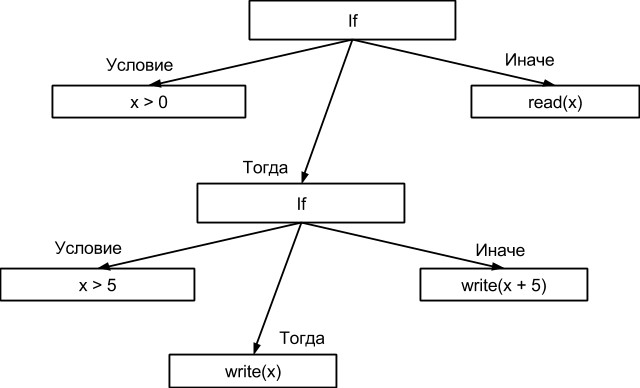
\includegraphics[width=0.6\textwidth]{nestedIf}
	\caption{Пример дерева “\lstinline{if-then-else}”}
	\label{fig:nestedIf}
\end{figure}

\begin{figure}[h!]
	\centering
	\lstinputlisting{Podkopaev/codes/nestedIf.l}
	\caption{Представление с помощью шаблонов с рис. \ref{fig:ifTmplt}}
	\label{fig:nestedIfCode}
\end{figure}

Одним из неочевидных свойств шаблонов является то, что с их помощью можно выражать не только базовые конструкции языка.
Например, можно завести отдельный шаблон для случая, когда обе ветки конструкции “\lstinline{if-then-else}” представляют собой операторы “\lstinline{write}” (см. рис. \ref{fig:writeNestedInIf}). Если добавить такой шаблон, то пример дерева с рисунка~\ref{fig:nestedIf} получит новое представление (см. рис. \ref{fig:nestedIfNew}).

\begin{figure}[h!]
	\lstinputlisting{Podkopaev/codes/writeNestedInIf.t}
	\caption{Пример задания шаблона для сложной конструкции}
	\label{fig:writeNestedInIf}
\end{figure}

\begin{figure}[h!]
	\lstinputlisting{Podkopaev/codes/nestedIfNew.l}
	\caption{Представление дерева с рис. \ref{fig:nestedIf} с использованием шаблона с рис. \ref{fig:writeNestedInIf}}
	\label{fig:nestedIfNew}
\end{figure}

\subsection{Построение образцов}

Для работы принтера неообходимо иметь возможность сравнивать синтаксическое представление шаблонов с деревом, которое печатается. Поэтому необходим синтаксический анализатор, который может разбирать шаблонные конструкции в рамках целевого языка. Удобным способом разработать данный анализатор является использование расширяемого синтаксического анализатора целевого языка. В результате работы расширенного анализатора получается набор образцов. В узлах синтаксического дерева, соответствующих меткам шаблонов, хранится информация о положении метки внутри текста образца, чтобы на этапе печати документа знать, куда вставлять представления поддеревьев.

\subsection{Печать дерева с использованием набора образцов}

На этапе, когда уже имеются необходимые образцы, происходит их сопоставление с синтаксическим деревом, переданным на печать.
Псевдокод алгоритма приведен ниже (см. рис. \ref{fig:comparePseudoCode}).

\begin{figure}[h!]
	\begin{algorithmic}
		\State{H --- ассоциативный массив, связывает деревья с их текстовым представлением}
		\State{M --- набор образцов для языковых конструкций}

		\State{ }
		\State{Комментарий: По дереву строит его текстовое представление}
		\Function{print}{$tree$}
			\If{$tree \in H$}
				\State\Return{$H[tree]$}
			\Else
				\State{Вызов print для поддеревьев $tree$}
				\State\Return{\Call{templateIter}{$tree$}}
			\EndIf
		\EndFunction

		\State{ }
		\State{Комментарий: Перебирает все образцы и пытается их применить к дереву}
		\Function{templateIter}{$tree$}
			\ForAll{$(templateTree, text) \in M$}
				\State{Комментарий: В случае исключения, переходит к новому элементу $M$}
				\State{$list$ := \Call{templateCompare}{$tree, templateTree$}}
				\State{$H[tree]$ := построенное представление для $tree$ по $list$ и $text$}
				\State\Return{$H[tree]$}
			\EndFor
		\EndFunction

		\State{ }
		\State{Комментарий: Возвращает список координат метки в тексте шаблона и соответствующее текстовое представление поддерева}
		\Function{templateCompare}{$tree, templateTree$}
			\If{$tree$ и $templateTree$ одного типа}
				\State{Вызвать $templateCompare$ для соответствующих поддеревьев}
				\State\Return{соединенный список результатов вызова для поддеревьев}
			\EndIf

			\If{$templateTree$ является меткой}
				\If{$H[tree]$ соответствует ограничениям метки}
					\State\Return{$[($координаты метки$, H[tree])]$}
				\Else
					\State{создать исключение}
				\EndIf
			\EndIf

			\State{Создать исключение, т.к. переданные деревья разной структуры}
		\EndFunction
		
	\end{algorithmic}
	\caption{Псевдокод сопоставления дерева с набором образцов}
	\label{fig:comparePseudoCode}
\end{figure}

Из псевдокода видно, что в случае, если для какого-нибудь поддерева не найдется соответствующий образец, то дерево невозможно будет напечатать. То есть множество образцов должно быть достаточным. Это естественное ограничение.

% Попробуем оценить время работы алгоритма. Пусть $|M|$ --- количество образцов, $height(T)$ --- высота дерева, а $K$ --- максимальное число поддеревьев у узла синтаксического дерева целевого языка. Тогда время работы алгоритма можно оценить как $O((|M| \times K)^{height(T)} )$.

Попробуем оценить время работы алгоритма. Для каждого узла дерева, переданного принтеру, вычисляется следующее:
\begin{enumerate}
	\item текстовое представление для детей;
	\item сравнение с имеющимися образцами;
	\item текстовое представление узла по выбранному образцу и представлениям детей.
\end{enumerate}

Текстовое представление вычисляется для каждого узла один раз. Сравнение с образцами занимает $O(B \times |M|)$ времени, где $B$ --- максимальное число узлов в дереве образца, а $|M|$ --- количество образцов. Построение текстового представления по выбранному образцу занимает $O(A)$, где $A$ --- максимальное количество меток в шаблоне, но так как очевидно, что $A \leq B$, то оценку можно заменить на $O(B)$. Таким образом, оценка на работу алгоритма для дерева с $T$ узлами равна $O(T \times B \times |M|)$.

Для сравнения, если реализовать аналогичный принтер с помощью библиотеки Азеро и Свиерстры, то это приведет к экспоненциальному от размера дерева расчету текстового представления. В случае библиотек Хьюза и Вадлера похожий принтер будет иметь квадратичную сложность.

\subsection{Реализованный принтер}

Описанный подход был реализован на примере принтера языка L, написанного на языке OCaml\footnote{http://ocaml.org}. Для написания синтаксического анализатора была использована библиотека Ostap\footnote{http://oops.math.spbu.ru/projects/ostap}.

В качестве примера работы принтера с разными шаблонами рассмотрим уже упоминавшуюся программу быстрого возведения в степень (см. рис. \ref{fig:lEx}).
С помощью шаблонов, приведенных в приложении~\ref{app:1}, принтер печатает программу в виде, изображенном на рисунке \ref{fig:firstTemplatePow}.

\begin{figure}[h!]
	\lstinputlisting{Podkopaev/codes/firstTemplatePow.l}
	\caption{Программа быстрого возведения в степень на языке L, напечатанная с помощью шаблонов из приложения~\ref{app:1}}
	\label{fig:firstTemplatePow}
\end{figure}

Шаблоны, приведенные в приложении~\ref{app:2}, представляют программу несколько иным образом (см. рис. \ref{fig:secondTemplatePow}).

\begin{figure}[h!]
	\lstinputlisting{Podkopaev/codes/secondTemplatePow.l}
	\caption{Программа быстрого возведения в степень на языке L, напечатанная с помощью шаблонов из приложения~\ref{app:2}}
	\label{fig:secondTemplatePow}
\end{figure}

Из приведенных примеров виден один из недостатков реализации. Если присмотреться к конструкции \lstinline{if-then-else}, то можно заметить, что \lstinline{then} и \lstinline{else} находятся на разных уровнях. Естественно, это нежелательный результат. Пока эта проблема не решена, в дальнейшем планируется разобраться с этой проблемой путем расширения языка шаблонов.

\section*{Заключение}

В рамках данной работы были изучены основные подходы к построению принтеров на основе функциональных языков и
разработан новый подход к заданию принтера целевого языка с помощью шаблонов. Данный подход апробирован для модельного языка L. 

В рамках развития работы планируется создать библиотеку для языка OCaml, которая позволит строить принтеры с помощью описанного
подхода.

% \bibliographystyle{plain}
% \bibliography{articles}

\begin{thebibliography}{99}
\bibitem{hughes} Hughes J. The Design of a Pretty-printing Library. Advanced Functional Programming. Springer Verlag, 1995.
\bibitem{oppen} Oppen D. Pretty Printing. Stanford Verification Group. Report No. 13. Computer Science Department Report No. STAN-CS-79-770, 1979.
\bibitem{wadler} Wadler P. A Prettier Printer. Journal of Functional Programming. Palgrave Macmillan, 1998.
\end{thebibliography}

\appendix
\section{Первый вариант набора шаблонов для языка L}
\label{app:1}
\lstinputlisting{codes/l_template.t}

\newpage

\section{Второй вариант набора шаблонов для языка L}
\label{app:2}

\lstinputlisting{codes/l_template_2.t}
